\documentclass[man]{apa7}

\input{includes/preamble_common}
\input{includes/preamble_apa7}

\title{Integración de patrones de diseño y paradigmas de desarrollo en proyectos de software gestionados con Scrum}
\shorttitle{Integración de patrones y paradigmas en Scrum}
\authorsnames{Autor: Jhampier Santos Ortiz, Instructor: Jesús Ariel González Bonilla}
\authorsaffiliations{Análisis y Desarrollo de Software, SENA}
\authornote{ORCID: 0009-0005-7050-2633. Correo: ortizjhampier@gmail.com. Ficha: 2899747. Fecha: 26 de septiembre de 2025}

\abstract{El presente artículo examina la relevancia y la interacción de cinco componentes fundamentales en el desarrollo de software contemporáneo: Git y GitHub, la Guía de Scrum 2020, los patrones de diseño, el patrón Modelo-Vista-Controlador (MVC) y el lenguaje de programación Java. Se adopta un enfoque descriptivo y analítico para mostrar cómo estas herramientas, metodologías y arquitecturas favorecen la colaboración, la trazabilidad y la calidad del código en proyectos de diversa escala. A lo largo del estudio se destaca que Git, combinado con la plataforma GitHub, asegura un control de versiones eficiente y un trabajo en equipo distribuido. Asimismo, la aplicación de Scrum según la guía 2020 promueve iteraciones cortas, transparencia y adaptabilidad a los cambios. Por su parte, los patrones de diseño y el patrón MVC refuerzan la modularidad, la reutilización de componentes y la separación de responsabilidades, mientras que Java aporta portabilidad, robustez y un ecosistema amplio que facilita la construcción de soluciones escalables. Los resultados de este análisis demuestran que la integración coordinada de estas prácticas constituye una base sólida para proyectos académicos y profesionales, incrementando la eficiencia, la mantenibilidad y la capacidad de respuesta frente a las demandas del entorno tecnológico actual.}

\keywords{Git, GitHub, Scrum 2020, patrones de diseño, MVC, Java}

\begin{document}
\maketitle

\section{Introducción}
El desarrollo de software actual se enfrenta a una rápida evolución tecnológica y a proyectos cada vez más complejos, lo que exige soluciones que garanticen escalabilidad, calidad y una colaboración eficaz entre equipos distribuidos. Estos retos influyen directamente en la estabilidad del código y en su capacidad de adaptación a lo largo del tiempo. Ante este panorama, la comunidad profesional y académica ha promovido el uso de herramientas y metodologías que faciliten la organización del trabajo y la trazabilidad de los cambios.

Dentro de este marco, el sistema de control de versiones Git y la plataforma colaborativa GitHub se han consolidado como pilares para la gestión de código, permitiendo registrar, revertir y coordinar modificaciones de forma segura. Paralelamente, la Guía de Scrum 2020 refuerza el enfoque ágil mediante ciclos de trabajo cortos e iterativos que impulsan la transparencia, la mejora continua y la entrega de valor en cada fase del proyecto. En el ámbito de la arquitectura de software, los patrones de diseño ofrecen soluciones probadas a problemas recurrentes, fomentando la modularidad y la reutilización del código, mientras que el Modelo-Vista-Controlador (MVC) establece una clara separación de responsabilidades que facilita el mantenimiento y la escalabilidad de las aplicaciones. Finalmente, el lenguaje Java, con su orientación a objetos y su portabilidad, se mantiene como una de las opciones más robustas y versátiles para el desarrollo de aplicaciones web, móviles y empresariales. En este contexto, el presente trabajo analiza y articula estos cinco elementos clave con el propósito de demostrar que su integración fortalece la calidad, la colaboración y la capacidad de respuesta en proyectos de software, ofreciendo un modelo de buenas prácticas aplicable en entornos académicos y profesionales.
\section{Fundamentación Teórica}
\subsection{Git and Github}
Git es un sistema de control de versiones distribuido que permite a los desarrolladores gestionar y registrar cada cambio en el código de forma eficiente, segura y con un historial completo de modificaciones. Su arquitectura distribuida posibilita que cada colaborador tenga una copia íntegra del repositorio, lo que incrementa la resiliencia del proyecto y facilita el trabajo sin conexión. GitHub, construido sobre Git, es una plataforma colaborativa en la nube que agrega herramientas para la revisión de código, la gestión de incidencias, las solicitudes de extracción (pull requests) y la integración y entrega continuas. Esta combinación promueve la trazabilidad de cambios, el trabajo organizado en ramas, la colaboración global en proyectos de cualquier escala y la automatización de flujos de desarrollo, contribuyendo a una mayor calidad y velocidad en la entrega de software \cite{ref1}.

\subsection{Scrum}
Scrum es un marco de trabajo ágil para la gestión de proyectos que se fundamenta en ciclos iterativos e incrementales llamados sprints, durante los cuales el equipo planifica, desarrolla y revisa funcionalidades concretas. La versión 2020 de la Guía Scrum refuerza la idea de auto-gestión del equipo, destacando la necesidad de que sus miembros asuman colectivamente la planificación y la responsabilidad de los resultados. También subraya la simplicidad y claridad de sus artefactos principales Product Backlog, Sprint Backlog e Incremento como medio para mantener la transparencia y facilitar el seguimiento del progreso. Los roles esenciales de Scrum Master, Product Owner y Equipo de Desarrollo se definen con mayor precisión para garantizar la comunicación constante y la eliminación de impedimentos. La aplicación de estos principios no solo mejora la adaptabilidad y la capacidad de respuesta ante cambios, sino que también promueve la entrega continua de valor y una cultura de mejora permanente dentro de los proyectos de software \cite{ref2}.

\subsection{Patrones de Diseño}
Los patrones de diseño constituyen soluciones probadas y ampliamente documentadas para resolver problemas recurrentes que surgen durante el desarrollo de software. Se dividen de manera general en tres grandes categorías: creacionales, que se enfocan en la instanciación flexible de objetos; estructurales, que facilitan la composición y relación entre clases y objetos; y de comportamiento, que se centran en la comunicación y asignación de responsabilidades entre componentes. Su propósito principal es favorecer la reutilización de código, la escalabilidad y la mantenibilidad de los sistemas, proporcionando a los desarrolladores un conjunto de guías que ayudan a construir arquitecturas más limpias, coherentes y fáciles de comprender. Además, su adopción fomenta buenas prácticas de programación y acelera la fase de diseño, al ofrecer soluciones previamente validadas por la comunidad de ingeniería de software \cite{ref3}.

\subsection{Modelo-Vista-Controlador (MVC)}
El patrón Modelo–Vista–Controlador (MVC) organiza una aplicación en tres componentes bien definidos. El Modelo se encarga de la lógica de datos y de las reglas de negocio, garantizando la integridad y el acceso a la información. La Vista gestiona la presentación, mostrando al usuario la interfaz y actualizándose conforme cambian los datos. El Controlador actúa como intermediario, recibiendo las acciones del usuario, procesando las solicitudes y dirigiendo el flujo entre el Modelo y la Vista. Esta separación de responsabilidades permite desarrollar, probar y mantener cada capa de manera independiente, favoreciendo la escalabilidad y facilitando la incorporación de nuevas funcionalidades sin afectar el resto del sistema. Además, el MVC mejora la legibilidad del código y promueve la reutilización de componentes, cualidades esenciales en proyectos de mediana y gran envergadura \cite{ref4}.

\subsection{Java}
Java es un lenguaje de programación orientado a objetos ampliamente utilizado en el desarrollo de aplicaciones web, móviles, de escritorio y empresariales. Se distingue por su portabilidad, posibilitada por la Máquina Virtual de Java (JVM), que permite ejecutar el mismo programa en diferentes plataformas sin modificaciones. Además, ofrece características de robustez, seguridad y manejo automático de memoria, lo que reduce errores y mejora la estabilidad de los sistemas. Su extenso ecosistema incluye frameworks y librerías como Spring, Hibernate y JavaFX, que facilitan el desarrollo ágil y escalable, así como herramientas de compilación y automatización que optimizan el ciclo de vida del software. Gracias a su comunidad global activa y a su evolución constante, Java sigue siendo una de las tecnologías preferidas para proyectos de gran envergadura que requieren fiabilidad y rendimiento \cite{ref5}.
\section{Metodología}
El presente proyecto se desarrolló bajo un enfoque cualitativo, orientado a la comprensión e interpretación de conceptos vinculados con Git y GitHub, la Guía de Scrum 2020, los patrones de diseño, el patrón Modelo–Vista–Controlador (MVC) y el lenguaje Java. Desde el inicio de la investigación se definió que estas tecnologías y metodologías representarían la base teórica para proponer buenas prácticas en el desarrollo de software colaborativo y escalable. Con el fin de sustentar y validar estas elecciones, se llevó a cabo un proceso de búsqueda, selección y análisis de literatura académica y técnica que ofreciera evidencia de sus beneficios y casos de uso. Se consideró fundamental identificar no solo la aplicabilidad individual de cada tema, sino también las sinergias que surgen al integrarlos en proyectos de diversa magnitud.

\subsection{Fase 1 - Recolección y construcción del thesaurus}
• Se utilizó como fuente principal Google Scholar, complementada con repositorios de documentación oficial y publicaciones especializadas. Se realizaron consultas con palabras clave relacionadas: Git, GitHub, Scrum 2020, patrones de diseño, MVC y Java.

• Cada recurso relevante fue documentado en un archivo "Thesaurus" con campos estandarizados que incluían término, fecha, fuente y nombre del artículo o guía consultada.

• El objetivo de esta fase fue reunir evidencia científica y técnica que respaldara el uso de estas herramientas y enfoques, proporcionando una base sólida para las recomendaciones metodológicas y prácticas presentadas en este trabajo.

\subsection{Fase 2 - Análisis cualitativo de la evidencia (síntesis del thesaurus)}
• El objetivo de esta fase fue transformar la información recopilada en argumentos sólidos que justificaran la elección de Git y GitHub, la Guía de Scrum 2020, los patrones de diseño, el patrón MVC y el lenguaje Java como elementos clave en el desarrollo de software. Para ello se realizaron lecturas críticas, resúmenes comparativos y reflexiones sobre cada fuente, evaluando aspectos como la colaboración distribuida, la trazabilidad de cambios, la modularidad de las arquitecturas y la portabilidad del código.

• La evidencia analizada confirmó la pertinencia de integrar estas tecnologías y metodologías en un mismo proyecto, destacando que su uso conjunto favorece la escalabilidad, la calidad del producto final y la eficiencia del trabajo en equipo. Asimismo, proporcionó lineamientos prácticos que orientan tanto el diseño de la arquitectura como la implementación y el mantenimiento de sistemas modernos.
\section{Diseño y desarrollo del sistema}
En esta etapa se transformaron los criterios teóricos y metodológicos en un sistema funcional, integrando de manera práctica el uso de Git y GitHub, la Guía de Scrum 2020, los patrones de diseño, el patrón Modelo–Vista–Controlador (MVC) y el lenguaje Java como ejes de construcción y organización del proyecto.

\subsection{Procedimiento detallado}
\subsubsection{Diseño de la arquitectura (MVC)}
Se definieron las capas principales del sistema: Modelo, encargado de la gestión de datos y la lógica de negocio; Vista, responsable de las interfaces de usuario; y Controlador, que coordina la comunicación entre ambos. Esta separación de responsabilidades permitió aumentar la mantenibilidad y la escalabilidad, facilitando la evolución independiente de cada componente.

\subsubsection{Patrones de Diseño}
Se aplicaron patrones creacionales y estructurales para optimizar la reutilización de código y garantizar una arquitectura clara y flexible. Esta práctica redujo la duplicación y facilitó la incorporación de nuevas funcionalidades.

\subsubsection{Lenguaje Java}
El desarrollo principal se realizó en Java, aprovechando su orientación a objetos, su portabilidad mediante la JVM y su amplio ecosistema de librerías. Se emplearon principios de encapsulamiento, herencia y polimorfismo para asegurar un código robusto y extensible.

\subsubsection{Scrum}
El equipo trabajó en sprints definidos, con reuniones de planificación, revisiones y retrospectivas. La auto-gestión y la transparencia recomendada por la guía 2020 permitieron ajustar prioridades y detectar incidentes de forma temprana, fomentando la mejora continua.

\subsubsection{Git and Github}
Todo el código se gestionó con Git y se alojó en GitHub, lo que brindó trazabilidad, trabajo en ramas, revisiones mediante pull requests y una integración continua eficaz para cada entrega.

\subsection{Herramientas complementarias}
• Backend: Java con Spring Boot, elegido por su seguridad y escalabilidad.

• Frontend web: React.js, por su flexibilidad en interfaces dinámicas.

• Aplicación móvil: React Native, para extender funcionalidades a entornos móviles sin duplicar código.

• Base de datos: PostgreSQL, encargada del manejo de la información de usuarios, eventos y reservas.

Esta fase consolidó la integración de herramientas, metodologías y arquitecturas, permitiendo obtener un sistema moderno, escalable y alineado con las mejores prácticas del desarrollo de software.
\section{Resultados}
Una vez concluido el análisis cualitativo, se determinó que el desarrollo de un sistema moderno requiere apoyarse en una combinación equilibrada de herramientas, metodologías y lenguajes que aseguren organización, escalabilidad y colaboración efectiva. En este sentido, se confirmó la relevancia de contar con un control de versiones robusto mediante Git y GitHub, así como de aplicar un marco ágil bien estructurado como la Guía de Scrum 2020, que permite adaptarse a los cambios, mejorar la comunicación entre los participantes y facilitar la entrega incremental de funcionalidades. Estos hallazgos orientaron las decisiones técnicas adoptadas y proporcionaron lineamientos prácticos para optimizar el trabajo en equipo y la calidad del producto final.

\subsection{Resultados en la arquitectura y el desarrollo del sistema}
Se implementó un software basado en el patrón Modelo–Vista–Controlador (MVC), el cual facilitó una clara separación de responsabilidades entre la lógica de negocio, la interfaz de usuario y la gestión de las interacciones. De forma complementaria, la aplicación de patrones de diseño aportó soluciones comprobadas para problemas comunes, incrementando la reutilización y la flexibilidad de la estructura. El lenguaje Java, elegido como núcleo del desarrollo, ofreció robustez, portabilidad y un amplio ecosistema de librerías, mientras que el uso de Git y GitHub garantizó la trazabilidad de los cambios y la colaboración distribuida del equipo. En conjunto, estos elementos permitieron construir un sistema escalable, seguro y alineado con las mejores prácticas del desarrollo de software contemporáneo.

\begin{figure}[htbp]
    \centering
    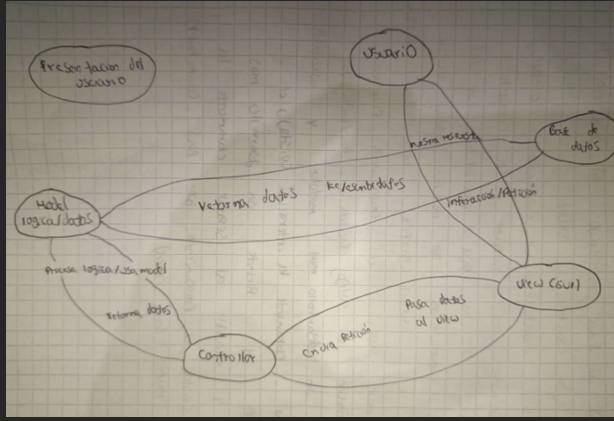
\includegraphics[width=0.5\textwidth]{graphics/MVC-patron.png}
    \caption{Modelo vista controlador}
    \label{fig:mvc}
\end{figure}

En la Figura \ref{fig:mvc} se presenta el diagrama de la arquitectura Modelo–Vista–Controlador (MVC) utilizada en el desarrollo del sistema. Esta representación muestra la interacción entre el Modelo, que gestiona la lógica de datos, el Controlador, encargado de coordinar las solicitudes del usuario, y la Vista, responsable de la presentación. El uso de MVC favoreció una organización clara del código y facilitó la incorporación de nuevas funcionalidades, permitiendo que las actualizaciones en cada componente se realicen sin afectar de manera negativa al resto de la aplicación.

\subsection{Resultados en la aplicación de la metodología ágil (Scrum)}
Durante el año académico se aplicaron los principios de Scrum en tres proyectos diferentes, manteniendo un registro continuo de avances y evidencias que demuestran la participación activa en cada uno de ellos. A continuación, se detallan los aportes y las pruebas de trabajo:

• \textbf{Odimo – Plataforma de domicilios}

Rol y aportes: desarrollo del backend, diseño de mockups en Figma y elaboración de documentación.

Evidencias: repositorio en GitHub con commits de las funcionalidades implementadas y material de soporte en Microsoft Teams.

URL de evidencia:

Github: \url{https://github.com/Darwin-9/Odimo.git}

Figma: \url{https://www.figma.com/design/lmqPj5pLqUQrRX6R1vQPms/Untitled?node-id=0-1&t=up4yA4ZGq39i7p2n-1}

Teams-Documentación: ADSO 2899747 - Documents - Soporte - All Documents

• \textbf{Sistema de Gestión de Inventario}

Rol y aportes: finalización de la documentación, desarrollo del backend funcional y comienzo del frontend, además de algunos mockups.

Evidencias: código y commits en GitHub, así como archivos de prueba y avances documentados en Microsoft Teams.

URL de evidencia:

Github: \url{https://github.com/Darwin-9/InventorySystem.git}

Figma: \url{https://www.figma.com/design/V89kbquYJic3yF700ZFP2K/Untitled?node-id=0-1&t=Y1Rj5pGSEjQQrcCH-1}

Teams-Documentación: Grupo 8- Gestión de Inventario ODIMO CANCELADO

• \textbf{Tu-Evento – Proyecto actual}

Rol y aportes: contribuciones activas en documentación, código y mockups, evidenciadas por los commits realizados y el trabajo colaborativo con el equipo.

Evidencias: historial de commits en GitHub y material compartido con los compañeros que confirma la participación en las diferentes fases del proyecto.

URL de evidencia:

Github: \url{https://github.com/lozano2303/tu-evento.git}

Figma: \url{https://www.figma.com/design/iuw3YMS7t81m3hIKMAvtHf/Tu-Evento?node-id=0-1&t=kUGHUgTCtokrMqo6-1}

Teams-Documentación: Grupo 5- Tu evento

\begin{figure}[htbp]
    \centering
    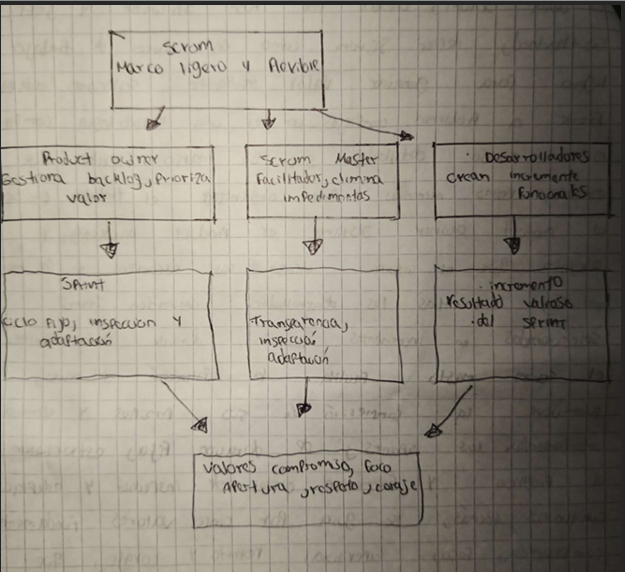
\includegraphics[width=0.5\textwidth]{graphics/scrum.png}
    \caption{Evidencias de trabajo colaborativo}
    \label{fig:evidencias}
\end{figure}

En la Figura \ref{fig:evidencias} se presentan las principales plataformas que sirvieron como soporte para la planificación, el seguimiento de avances y la entrega de resultados en los tres proyectos desarrollados durante el año. En lugar de un tablero de Trello, la organización y control de tareas se documentaron directamente en GitHub, Figma y Microsoft Teams, donde se registran commits, diseños, documentación y mensajes de comunicación del equipo.
\section{Conclusión}
A partir de la metodología cualitativa aplicada en este proyecto, se comprobó que la integración de herramientas de control de versiones, metodologías ágiles, arquitecturas de software y lenguajes robustos es esencial para el éxito en el desarrollo de sistemas. El análisis documental y las evidencias prácticas permitieron identificar como pilares fundamentales a Git y GitHub, la Guía de Scrum 2020, los patrones de diseño, el patrón Modelo–Vista–Controlador (MVC) y el lenguaje Java, cada uno aportando ventajas específicas para la organización, la colaboración y la escalabilidad de los proyectos. Los resultados obtenidos demuestran que el uso de Git y GitHub garantizó la trazabilidad de cambios y el trabajo colaborativo; Scrum 2020 fortaleció la planificación, la comunicación y la entrega incremental de funcionalidades; los patrones de diseño y la arquitectura MVC facilitaron la estructura clara del sistema; y Java proporcionó robustez, portabilidad y un ecosistema amplio para el desarrollo. En conjunto, estos hallazgos evidencian que la combinación de una base teórica sólida con la práctica constante en los tres proyectos realizados durante el año permitió obtener productos funcionales y alineados con las necesidades planteadas, confirmando la eficacia de esta integración de tecnologías y metodologías en entornos académicos y profesionales.
\input{sections/A1_apendices}

\printbibliography

\end{document}